% MODELAGEM MATEMÁTICA PARA A OTIMIZAÇÃO DO EQUILÍBRIO SÓLIDO-LÍQUIDO------------------------------------------------------------------

\chapter{MODELAGEM MATEMÁTICA}
\label{chap:modelagem_matematica}

\section{Otimização}

O conceito de \textit{otimização} é uma forma de trazer uma solução satisfatória para problemas complexos que exigem a tomada de decisão ou alocação. Problema de decisão complexa, obtendo quantidade expressiva de valores correlacionadas com várias variáveis, foca-se em único objetivo projetado para quantificar o desempenho e medir a qualidade da decisão. Esse objetivo pode ser maximizado ou minimizado como as devidas restrições que pode limitar a seleção dos valores das variáveis de decisão e ajudar em sua escolha, como o objetivo de lucro ou perda em um ambiente de investimento ou de bem estar social. \cite{Luenberger2016}

\section{Programação Não Linear}

Problemas reais são na grande maioria formulados por restrições, como a política de produção em uma grande empresa ou planejamento da agência governamental, são problemas de programação não linear com restrições.

Em geral o problema de programação é indicada por:
\begin{equation}
\begin{array}{rcccc}
\mbox{minimização} & f(x) & & & \\
\mbox{sujeita as condições} & h_{i}(x)&=&a_{i}, & i=1,2,\ldots,m \\
& g_ {j}(x)&\leq&b_j, & j=1,2,\ldots,p\\
& x\in S & & & \\
\end{array}
\end{equation}

Em que $x$ é um vetor n-dimensional $x=(x_{1},x_{2},\ldots,x_{n})$, $f_{i}$ e $h_i$ são funções reais das variáveis $x_{1},x_{2},\ldots,x_{n}$. A função $f$ é a \textit{função objetivo}, $g$, $h$ e o conjunto $S$ são as restrições do problema; com os parâmetros $a_i$ e $b_j$. \cite{Luenberger2016, Rocha2009a}

\section{Convexidade}

Os conceitos relacionados aos conjuntos \textit{convexos} são relevantes teoria da otimização, representada pela Figura \ref{fig:convexSet} na forma bidimensional, que por sua vez é essencial para um estudante de otimização ter conhecimento de suas propriedades mais fundamentais. \cite{Luenberger2016, Rocha2009a}

\begin{definicao}
	Dado um conjunto $C\subset E^{n}$ diz que é \textbf{convexo} se para qualquer $x_{1}, x_{2} \in C$ e para todo $\alpha\in\mathbb{R}$, tal que o ponto $\alpha x_{1}+(1-\alpha)x_{2}\in C$.
\end{definicao}

%\begin{comment}
\begin{figure}[H]
	\centering
	\subbottom[Convexo]{
		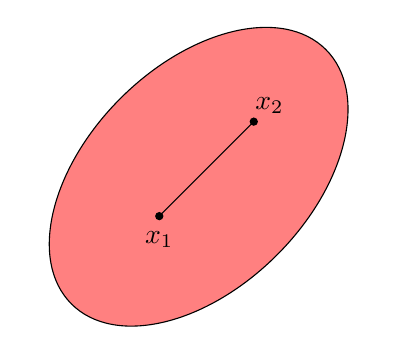
\begin{tikzpicture}
		\draw[rotate=-45,fill=red!50] (0,0) ellipse (40pt and 65pt);
		\draw (-0.5,-0.5) -- (0.7,0.7);
		\fill (-0.5,-0.5) circle[radius=1.5pt];
		\fill (0.7,0.7) circle[radius=1.5pt];
		\node at (-0.5,-0.8) {$x_1$};
		\node at (0.9,0.9) {$x_2$};
		\end{tikzpicture}}
	\hspace{2cm}
	\subbottom[Não Convexo]{
		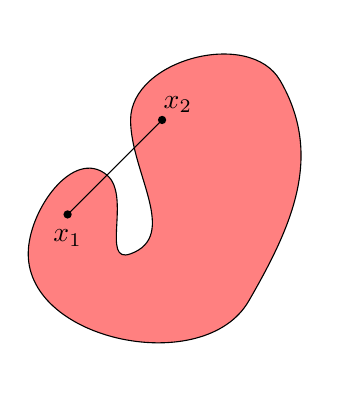
\begin{tikzpicture}
		\draw[fill=red!50] (0,0) to [out=140,in=90] (-1,-1)
		to [out=-90,in=240] (1.8,-1.6)
		to [out=60,in=-60] (2.2,1.2)
		to [out=120,in=90] (0.3,0.7)
		to [out=-90,in=20] (0.3,-1)
		to [out=200,in=-40] (0,0);
		\draw (-0.5,-0.5) -- (0.7,0.7);
		\fill (-0.5,-0.5) circle[radius=1.5pt];
		\fill (0.7,0.7) circle[radius=1.5pt];
		\node at (-0.5,-0.8) {$x_1$};
		\node at (0.9,0.9) {$x_2$};
		\end{tikzpicture}}
	\caption{Convexidade de conjuntos}
	\label{fig:convexSet}
\end{figure}

\section{\textit{Softwares} Utilizados}

Os \textit{softwares} utilizados para o desenvolvimento do trabalho, foram descritos nos subitens que seguem.

% TODO GEOGEBRA

\subsection{\textit{Geogebra}}
Para a coleta de pares ordenados e organização das misturas binárias para fins de cálculos vamos utilizar o \textit{software} \textit{Geogebra}\footnote{Site do Geogebra \url{https://www.geogebra.org/}} é um \textit{software} de código aberto Figura \ref{fig:11}, oferecido para várias plataformas, com a finalidade didática e de pesquisa. 
\begin{figure}[H]
	\centering
	\includegraphics[width=0.9\linewidth 
	%,height=0.4\textheight
	]{dados/figuras/Geogebra_1.png}
	\caption[Site do Geogebra]{Site do Geogebra}
	\label{fig:11}
\end{figure}

\subsection{\textit{GAMS} General Algebric Model System}

O \textit{software} \textit{GAMS}\footnote{Site do GAMS \url{https://www.gams.com/}} é uma sistema de modelagem algébrica, desenvolvido para determinar soluções de sistemas com algoritmos matemáticos e otimização Figura \ref{fig:14}. O \textit{software} \textit{GAMS} com \textit{solver} comercial, para resolver modelos com aplicações em grande escala, com pacotes de testes \textit{GAMS} fornece modelos algébrico em código C, Delphi, Java e Fortran. 

\begin{figure}[H]
	\centering
	\includegraphics[width=1.0\linewidth 
	%,height=0.4\textheight
	]{dados/figuras/Gams_1.png}
	\caption[Site do \textit{GAMS}]{Site do \textit{GAMS}}
	\label{fig:14}
\end{figure}

\subsection{\textit{PyCharm} e \textit{R}}

Os \textit{software} \textit{PyCharm}\footnote{Site do \textit{PyCharm} \url{https://www.jetbrains.com/pt-br/pycharm/}} (FIGURA \ref{fig:15}) possui licença gratuita com restrições, disponíveis para as principais plataformas e, conjuntamente com a utilização da biblioteca \textit{R}\footnote{A base de dados para implementação de modelos estatísticos disponível no site \url{https://cran.r-project.org/}} (FIGURA \ref{fig:16}), se apresentam como uma base para implementação de algoritmos e modelos estatísticos. 

O \textit{PyCharm} possui uma IDE (Ambiente de Desenvolvimento Integrado) completa e simples para realizar o trabalho. A integração das bibliotecas ou  \textit{plugins} do \textit{software} traz melhor experiência, possui muitos tutoriais para melhor encaminhamento. Para esse trabalho, este \textit{software} foi usado na construção dos diagramas de fases junto com o \textit{R} para uma melhor perspectiva e pela facilidade de montar os algoritmos para tal aplicação. A biblioteca do \textit{R} auxiliou nos cálculos da Soma de Quadrado de Erro e no Coeficiente de Determinação forma dinâmica, contribuindo na escolha do modelo estatístico na comparação da técnica de DSC (Calorimetria Exploratória Diferencial) com os modelos termodinâmicos de Margules Simétrico, Margules Assimétrico e Wilson.
\begin{figure}[H]
	\centering
	\includegraphics[width=1.0\linewidth 
	%,height=0.4\textheight
	]{dados/figuras/Pycharm_1.png}
	\caption[Site do \textit{PyCharm}]{Site do \textit{PyCharm}}
	\label{fig:15}
\end{figure}
\begin{figure}[H]
	\centering
	\includegraphics[width=1.0\linewidth 
	%,height=0.4\textheight
	]{dados/figuras/R_1.png}
	\caption[Site do projeto R]{Site do projeto R}
	\label{fig:16}
\end{figure}

\subsection{Editor de texto \LaTeXe}

\LaTeXe  é o \textit{software} de código aberto de alta qualidade afim de produzir impressões profissionais e arquivos PDF, cuja base de dados \textit{TexLive}\footnote{Se encontra no site \url{http://tug.org/texlive/}} para plataformas Linux e macOS, organizada por \textit{TeX User Group} instituição sem fins lucrativos fundada em 1980, composto por \TeX\ \ criado por Donald Knuth e a mais conhecida ou difundida \textit{MikTex}\footnote{Se encontra no site \url{https://miktex.org/}} para todas as plataforma. A interface gráfica foi utilizado o \textit{TeXstudio}\footnote{Se encontra no site \url{https://www.texstudio.org/}} e \textit{Overleaf}\footnote{Se encontra no site \url{https://pt.sharelatex.com/}} uma ferramenta online para trabalhos colaborativos com o sistema de versionamento podendo ver quais são as modificações feitas por cada um colaborador. A a principal finalidade do \LaTeX é trazer uma tipografia de alta qualidade com o intuito trazer uma leitura mais agradável visualmente, com a biblioteca \textit{amsmath} para escrever fórmulas matemática, \textit{tikz} para criar desenhos vetoriais como os desenhos Figura\ref{fig:convexSet} e Figura\ref{fig:diagrama2}, \textit{chemformula} para fórmulas químicas, colabora com citação, facilita indexação de elementos e entre outras funcionalidades. \cite{latexchemformula,latexabntex2,latextikz,tex}

\begin{figure}[H]
	\centering
	\includegraphics[width=1.0\linewidth 
	%,height=0.4\textheight
	]{Miktex.png}
	\caption[Miktex]{Miktex}
	\label{fig:Miktex}
\end{figure}

\section{Modelos Matemáticos para a Programação Não-Linear}\label{subsection:1}

\hspace{5mm}Determinar a equação de estado que indica o equilíbrio sólido-liquido em um fluido puro a partir da equação molar da energia de \textit{Gibbs}.
\begin{equation}\label{eq:gibbs_2}
\gibbsm^{L}(T,P)=\gibbsm^{S}(T,P)
\end{equation}
como a energia de \textit{Gibbs} é definida por
\begin{equation}\label{eq:gibbs_3}
G\equiv H-TS
\end{equation}
em que $H$ é \textit{entalpia} e $S$ a \textit{entropia}. Derivando a equação \ref{eq:gibbs_3}, obtém-se,
\begin{equation}\label{eq:gibbs_4}
dG=-SdT+VdP
\end{equation}
de tal forma que
\begin{equation}\label{eq:gibbs_5}
\left(\dfrac{\partial G}{\partial T}\right)_{P}=-S
\end{equation}
e 
\begin{equation}\label{eq:gibbs_6}
\left(\dfrac{\partial G}{\partial P}\right)_{T}=V
\end{equation}

Agora integrando a equação \ref{eq:gibbs_6}, obtém-se duas pressões e temperatura constante, obtém-se
\begin{equation}\label{eq:gibbs_7}
G(T_1,P_2)-G(T_1,P_1)=\int_{P_1}^{P_2}VdP
\end{equation}
se o líquido considerado fosse um gás ideal $V^{GI}=\dfrac{RT}{P}$, tal que
\begin{equation}\label{eq:gibbs_8}
G^{GI}(T_1,P_2)-G^{GI}(T_1,P_1)=\int_{P_1}^{P_2}\dfrac{RT}{P}dP
\end{equation}
subtraindo a equação \ref{eq:gibbs_8} de \ref{eq:gibbs_7} obtém-se
\begin{equation}\label{eq:gibbs_9}
[G(T_1,P_2)-G^{GI}(T_1,P_2)]-[G(T_1,P_1)-G^{GI}(T_1,P_1)]=\int_{P_1}^{P_2}\left(V-\dfrac{RT}{P}\right)dP
\end{equation}
sendo assim, considerando $P_1=0$ para todo fluído são gases ideais para que $G(T_1,P=0)=G^{GI}(T_1,P=0)$, pode-se reescrever a equação \ref{eq:gibbs_9}.
\begin{equation}\label{eq:gibbs_10}
G(T,P)-G^{GI}(T,P)=\int_{0}^{P}\left(V-\dfrac{RT}{P}\right)dP
\end{equation}
\cite{Sandlel}

Donde que defini-se a função termodinâmica chamada de \textbf{fugacidade} e indica-se por $f$, definida por
\begin{equation}\label{eq:fugacidade_1}
f=P\mbox{exp}\left\{\dfrac{G(T,P)-G^{GI}(T,P)}{RT}\right\} =P\mbox{exp}\left\{\dfrac{1}{RT}\int_{0}^{P}\left(V-\dfrac{RT}{P}\right)dP\right\}
\end{equation}
em que o coeficiente de fugacidade é definido pela razão $\dfrac{f}{P}$ e é indicada por $\phi$.
\begin{equation}\label{eq:fugacidade_2}
\phi=\dfrac{f}{P}=\mbox{exp}\left\{\dfrac{G(T,P)-G^{GI}(T,P)}{RT}\right\} =\mbox{exp}\left\{\dfrac{1}{RT}\int_{0}^{P}\left(V-\dfrac{RT}{P}\right)dP\right\}
\end{equation}
A função fugacidade existe por uma relação com a energia molar de \textit{Gibbs} para o calculo do equilíbrio de fase. O critério do equilíbrio de duas fases é indicada na equação \ref{eq:gibbs_2} como $\gibbsm^{\mbox{I}}=\gibbsm^{\mbox{II}}$ com a restrição $T$ e $P$ constantes. Dessa equação junto com as equações \ref{eq:fugacidade_1} e \ref{eq:fugacidade_2}. 
\begin{equation}\label{eq:fugacidade_3}
\gibbsm^{GI}(T,P) + RT\ln\dfrac{f^{\mbox{I}}(T,P)}{P} = \gibbsm^{GI}(T,P) + RT\ln\dfrac{f^{\mbox{II}}(T,P)}{P}
\end{equation}
consequentemente a energia de \textit{Gibbs} molar do gás ideal em $T$ e $P$ constante possuem valores iguais, independente da fase utilizada a condição de equilíbrio é indicada
\begin{equation}\label{eq:fugacidade_4}
\ln\dfrac{f^{\mbox{I}}(T,P)}{P} = \ln\dfrac{f^{\mbox{II}}(T,P)}{P}
\end{equation}
em termos de fugacidade
\begin{equation}\label{eq:fugacidade_5}
f^{\mbox{I}}(T,P) = f^{\mbox{II}}(T,P)
\end{equation}
e o coeficiente de fugacidade
\begin{equation}\label{eq:fugacidade_6}
\phi^{\mbox{I}}(T,P) = \phi^{\mbox{II}}(T,P)
\end{equation}
No entanto para fins de cálculo é interessante troca-se a variável $P$ por $V$ uma vez que a pressão é uma constante, da equação \ref{eq:fugacidade_4} e para isso utiliza-se segundo SANDLEL \citeyear{Sandlel}
\begin{equation}\label{eq:fugacidade_7}
dP=\dfrac{1}{\underline{V}}d(P\underline{V})-\dfrac{P}{\underline{V}}d\underline{V}
\end{equation}
em que $\underline{V}$ é o volume molar e mudando a variável de integração obtém-se
\begin{equation}\label{eq:fugacidade_8}
\ln\dfrac{f(T,P)}{P} =\ln\phi = \int_{\underline{V}=\infty}^{\underline{V}}\left[\dfrac{RT}{\underline{V}}-P\right] d\underline{V}-\ln Z+(Z-1)
\end{equation}
quando $Z=\dfrac{P\underline{V}}{RT}$ é chamado de fator de compressão e para obter a equação geral do coeficiente de fugacidade, indicada por
\begin{equation}\label{eq:fugacidade_9}
\ln\dfrac{f(T,P)}{P} =\ln\phi = \int_{\underline{V}=\infty}^{\underline{V}}\left[\dfrac{RT}{\underline{V}}-P\right] d\underline{V}-\ln Z+(Z-1)
\end{equation}
\cite{Sandlel}

Mas para Energia de \textit{Gibbs} em uma mistura em função da temperatura, pressão molar de cada para cada espécie é representada pela diferencial total da função de energia de Gibbs como 
\begin{equation}\label{eq:mistura_1}
dG=-SdT+VdP+\sum_{i=1}^{C}\overline{G}_{i}dN_{i}
\end{equation}
%sandler pg 363 421 (8.2-1)

A energia molar de \textit{Gibbs} é conhecida como \textbf{potencial químico} representada por $\mu_i$, considere as equações para um fluido puro

\begin{equation}
    \frac{1}{N}\left(\frac{\partial G}{\partial P}\right)_{T,N}=\left(\frac{\partial\underline{G}}{\partial P}\right)_{T}=\underline{V}
\end{equation}
,
\begin{equation}
    \frac{1}{N}\left(\frac{\partial G}{\partial T}\right)_{P,N}=\left(\frac{\partial\underline{G}}{\partial T}\right)_{P}=-\underline{S}
\end{equation}
e
\begin{equation}
    \left(\frac{\partial G}{\partial N}\right)_{T,P}=-\underline{G}
\end{equation}

Uma vez que a entalpia pode ser escrita em função da entropia e pressão, segue as equações. 
Por definição $H=U+PV$, tal que
\begin{equation}
    \begin{array}{rcl}
        dH&=&dU+V dP+P dV = T dS - P dV + G dN + V dP + P dV \\
         & = & T dS + V dP + G dN
    \end{array}
\end{equation}
e para um sistema fechado
\begin{equation}
    d\underline{H} = T d\underline{S} + \underline{V} dP
\end{equation}
obtendo
\begin{equation}\label{eq:entalp1}
    \begin{array}{rcl}
        dH & = & \left(\dfrac{\partial H}{\partial P}\right)_{S,N_i}dP + \left(\dfrac{\partial H}{\partial S}\right)_{P,N_i}dS + \displaystyle\sum_{i=1}^{C}\left(\dfrac{\partial H}{\partial N_i}\right)_{P,S,N_{j\neq i}}dN_i  \vspace{3mm}\\
         & = & V dP + T dS + \displaystyle\sum_{i=1}^{C}\left(\dfrac{\partial H}{\partial N_i}\right)_{P,S,N_{j\neq i}}dN_i
    \end{array}
\end{equation}
no entanto, para $H = G + T S$ e Equação \ref{eq:entalp1}, obtém
\begin{equation}\label{eq:entalp2}
    \begin{array}{rcl}
        dH& = & dG + T dS + S dT = -S dT + V dP + \displaystyle\sum  \overline{G}_i dN_i + T dS + S dT\vspace{3mm}\\
          & = & V dP + T dS + \displaystyle\sum  \overline{G}_i dN_i
    \end{array}
\end{equation}

Comparando as Equações \ref{eq:entalp1} e \ref{eq:entalp2}, estabelece
\begin{equation}
    \left(\dfrac{\partial H}{\partial N_i}\right)_{P,S,N_{j\neq i}} = \overline{G}_i = \left(\dfrac{\partial G}{\partial N_i}\right)_{T,P,N_{j\neq i}}
\end{equation}
isto é, a derivada $\left(\dfrac{\partial H}{\partial N_i}\right)_{P,S,N_{j\neq i}}$ é igual a energia parcial molar de Gibbs .

De modo análogo estabelecido
\begin{equation}
    dU = T dS - P dV + \displaystyle\sum_{i}^{C} \overline{G}_i dN_i
\end{equation}
\begin{equation}
    dA = - P dV - S dT + \displaystyle\sum_{i}^{C} \overline{G}_i dN_i
\end{equation}
com
\begin{equation*}
    \overline{G}_i=\left(\dfrac{\partial U}{\partial N_i}\right)_{S,V,N_{j\neq i}}=\left(\dfrac{\partial A}{\partial N_i}\right)_{T,V,N_{j\neq i}}
\end{equation*}
Pode observar que a energia parcial molar de Gibbs assume um papel importante em misturas. 

Agora considere uma função termodinâmica em função de $\theta$ com propriedades molares
\begin{equation*}
    N\underline{\theta} =\sum N_i\overline{\theta}_i
\end{equation*}
derivando pela regra do produto
\begin{equation}\label{eq:ental4}
    d(N\underline{\theta}) = \sum N_i d\overline{\theta}_i + \sum  d\overline{\theta}_i d N_i
\end{equation}
Contudo a função $N\underline{\theta}$ com $T$, $P$ e números de mols.
\begin{equation}\label{eq:ental3}
    d(N\underline{\theta})= N\left(\dfrac{\partial \underline{\theta}}{\partial T}\right)_{P,N_{i}}dT + N\left(\dfrac{\partial \underline{\theta}}{\partial P}\right)_{T,N_{i}}dP+ \sum \overline{\theta}_idN_i
\end{equation}

Subtraindo as Equações \ref{eq:ental3} e \ref{eq:ental4} obtém-se a  \textbf{equação generalizada Gibbs-Duhem}.
\begin{equation}
    \displaystyle\sum_{i=1}^{C}N_id\overline{\theta}_i|_{T,P}=0
\end{equation}
e a equação de Gibbs-Duhem com $T$ e $P$ constantes.
\begin{equation}
    \displaystyle\sum_{i=1}^{C}x_id\overline{\theta}_i|_{T,P}=0
\end{equation}

Para misturas binárias 
\begin{equation}
    \displaystyle\sum_{i=1}^{2}x_i\left(\dfrac{\partial \underline{\theta}_1}{\partial x_1}\right)_{T,P}dx_1=0
\end{equation}

Determinando a equação de Gibbs-Duhem para misturas binárias com $T$ e $P$ constantes.

\begin{equation}
   x_1\left(\dfrac{\partial \underline{G}_1}{\partial x_1}\right)_{T,P}+ x_2\left(\dfrac{\partial \underline{G}_2}{\partial x_1}\right)_{T,P}=0
\end{equation}
usando $x_2=1-x_1$ e $dx_2=-dx_1$.

